\documentclass[12pt]{article}
\usepackage{geometry}
\geometry{left=1in,right=0.75in,top=1in,bottom=1in}

%%%%%%%%%%%%%%%%%%%%%%%%%%%%%%%%%%%%%%%%
% Replace ABCDEF in the next line with your chosen problem
% and replace 1111111 with your Team Control Number
\newcommand{\Problem}{C}
\newcommand{\Team}{2018915}
%%%%%%%%%%%%%%%%%%%%%%%%%%%%%%%%%%%%%%%%

\usepackage{newtxtext}
\usepackage{amsmath,amssymb,amsthm}
\usepackage{newtxmath} % must come after amsXXX
\usepackage{palatino}
\usepackage{booktabs}
\usepackage{algorithm}
\usepackage{algpseudocode}
\usepackage{graphics}
\usepackage{epsfig}
\usepackage{graphicx}
\usepackage{url}
\usepackage{hyperref}
\usepackage{subfigure}
\usepackage{enumitem}
\usepackage{listings}
\usepackage{color}
\usepackage{xcolor}
\usepackage{fancyhdr}
% \usepackage{inputenc}

\lhead{Team \Team}
\rhead{}
\cfoot{}

\newtheorem{theorem}{Theorem}
\newtheorem{corollary}[theorem]{Corollary}
\newtheorem{lemma}[theorem]{Lemma}
\newtheorem{definition}{Definition}

%%%%%%%%%%%%%%%%%%%%%%%%%%%%%%%%
\begin{document}
\graphicspath{{.}}  % Place your graphic files in the same directory as your main document
\DeclareGraphicsExtensions{.pdf, .jpg, .tif, .png}
\thispagestyle{empty}
\vspace*{-16ex}
\centerline{\begin{tabular}{*3{c}}
	\parbox[t]{0.3\linewidth}{\begin{center}\textbf{Problem Chosen}\\ \Large \textcolor{red}{\Problem}\end{center}}
	& \parbox[t]{0.3\linewidth}{\begin{center}\textbf{2020\\ MCM/ICM\\ Summary Sheet}\end{center}}
	& \parbox[t]{0.3\linewidth}{\begin{center}\textbf{Team Control Number}\\ \Large \textcolor{red}{\Team}\end{center}}	\\
	\hline
\end{tabular}}
%%%%%%%%%%% Begin Summary %%%%%%%%%%%
% Enter your summary here replacing the (red) text
% Replace the text from here ...
\begin{center}
    \textbf{Dig and Predict: Analysis of Amazon Reviews Data}
\end{center}

Sunshine Company is planning to release three new products in online market place: hair dryer, baby pacifier, and microwave oven. To help Sunshine company succeed in these three products, we conducted text-based, value-based, and time-based analysis of Amazon review data of three products.
%% Text Analysis
First, we divide the review body text into three groups corresponding to their ratings. We joined the words of these text with the Afinn list of English words to filter out words which do not have independent meanings. We then count the most frequent word within each group. We selected words with top five frequency of appearance and draw the word clouds to show their count. Combining them with the sentiment grade given by Natural Language Processing(NLP) method and original text, we concluded customer preference and crucial product features. 
%% Correlation Analysis

We then explore the relationships between attributes of the data sets. We calculate the correlation coefficient between six factors of each product's data set:length of review text, number of vine customers, count of verified purchases, proportion of helpful votes, star rating, and proportion of high rating among all review records. With the help of data visualization, we came to conclusion that, for all products, except for length of review texts, all other factors have different levels of positive correlation with star rating and proportion of high ratings among all. Star rating and the proportion of high ratings remain highly correlated. 

%% Time Series
Some researchers have revealed that customers are more willing to buy a product that with good ratings. In this study, we use two indicators to represent whether a product is popular and will be sold well. The first indicator is the average daily star ratings. The second indicator is the average daily good ratio, which describes whether a customer would like to give a good star rating. In order to predict those two indicators, a novel deep learning model Multi-Stacked Fully Connected Bidirectional Long-Short Term Memory model(MSFCB-LSTM), is proposed to predict the time series data. In this work, we define stacked bidirectional Long-Short Term Memory(LSTM) with two layers as the first temporal features or information abstraction, then connect with one layer LSTM to remedy potential temporal correlation.After stacked BiLSTM and LSTM, two Dense layers added at the end, which is capable of reasonably controlling dimensions in hidden layers output, and more precisely capture non-linearity between inputs and outputs since inputs in our model are multivariate with abstract correlations.

The results shows that our proposed model could predict the average daily good ratio well. Due to the deficiency of features, we could not predict the average daily star ratings as well as we predict the average daily good ratio. But the patters of the changes of the average daily star ratings could be well described. Moreover, we find that there exists an almost linear relationship between the average daily good ratio and the average daily star ratings. We could combine those two indicators together to predict and make final decisions.\\[2ex]
\textbf{Key Words:} Text Mining, MSFCB-LSTM, Time Series, NLP


\clearpage
\pagestyle{fancy}
% Uncomment the next line to generate a Table of Contents
%\tableofcontents 
\newpage
\setcounter{page}{1}
\rhead{Page \thepage\ }

% sheet %%%%%%%%%%%%%%%%%%%%%%%%%%%%%%%%%%%%%%%%%%%%%%%%%%%%%%%%%%%%
\tableofcontents

\section{Introduction}
\subsection{Background}

The e-commerce market has changed the way business is transacted, especially in the retail industry. As one of the biggest platform of e-commerce, Amazon has a complete system of customer rating and reviewing, which provides both retailers and future customers sufficient information for further marketing strategies as well as buying decisions. 

Recent years have seen an increasing amount of research
efforts expanded in understanding the textual review resources for Business use. The existing data set contains records of the three products: hair dryer, microwave, and pacifier As a company which is going to release these new product online, Sunshine Company seeks to explore these data and identify the market factors related with sales to increase competence. 

\subsection{Restatement of the Problem}
To develop a online strategy and identify the product features which customer value, it is necessary to combine time-based measures, text-based measures and data-based measure. We conclude specific tasks are as follows:
\begin{itemize}
	\item The appearance of words related to product features can be calculated and categorized according to rating, thus reflecting customers' preference and requirement. 
	\item Taking account of all the products within one kind, build a time series model to predict the products' future rating and the proportion of positive rating among all reviews. Our models consider the following factors: \\
	1. the number of verified reviews \\
	2. the number of vine customers\\
	3. the proportion of helpful reviews\\
	4. the total numbers of words in the rating text
	\item Evaluate the relationship between review factors and rating and proportion of positive ratings, identify the simulators for number of reviews and better rating trend. 
\end{itemize}
From the above analysis, we conclude the evaluation results. Based on the measurements, we propose strategies to Sunshine company with regard to desired product feature and online marketing. We then test the accuracy of the prediction model. Finally we analyze the strength and weakness of the existing model. 

\subsection{Given Data}
We were given three data sets which are hair dryer, microwave, and pacifier. Each data set is of the same form, consisting of product information and customer reviews within more than ten years. The data we will use are product ids, star ratings, votes, number of vine customers, verified purchases, review content and date.
During different time, many product have missing information, especially during earlier years, we set the missing values to null and ignore them when calculating sum and averages. 

\section{Assumptions and Terminology}
\subsection{Assumptions}
\begin{itemize}
    \item In time series analysis part, data of products with more than 50 records are considered valid
    \item The average rating of the product reflect the product's level of success
    \item The proportion of positive ratings among all reviews also reflects products' future trend of success
    \item The size of market is not considered during evaluation and prediction
    \item Potential social and economic factors are not considered in constructing the evaluation model
\end{itemize}

\subsection{Terminology}

\begin{table}[h!]
\centering
 \begin{tabular}{|| c c||} 
 \hline
 Meaning & Notation \\ [0.5ex] 
 \hline\hline
Average star rating on time t & $R_{S_{t}}$ \\[0.5ex]
Average good ratio on time t & $R_{G_{t}}$\\ [0.5ex]
Average proportion of helpful votes on time t & $p_{v_{t}}$\\[0.5ex]
Average number of words count in the review body on time t & $N_{word_{t}}$ \\[0.5ex]
Average number of verified purchase on time t & $N_{veri_{t}}$\\[0.5ex]
Average number of vine customers on time t & $N_{vine_{t}}$\\
 \hline
 \end{tabular}
\end{table}
\begin{itemize}
    \item Good ratio is proportion of good rating records among all review records, which is defined as follows:
    \begin{equation*}
        R_{G_{t}} = \dfrac{N_{G_{t}}}{N_{T_{t}}}
    \end{equation*}
    where $N_{G_{t}}$ represents the number of good star-rating (star-rating that is larger or equal to four) at time t, and $N_{T_{t}}$ represents the total number number of star-rating at time t.
    $R_{G_{t}}$ represents the ratio of people who is willing to give a good rate at time t. To predict $R_{G_{t}}$, we could conclude that whether a product is popular among customers.
    \item Proportion of helpful votes is number of helpful votes divided by total votes.
    \item Words count is number of words in the review body
    \item Each defined item above represents a daily average on day t.
\end{itemize}

\newpage
\section{Measurements and Characteristics of Review records}
\subsection{Data Processing}
Before setting up time series model, we selected out product records which have more than 50 review records. We analyze data of all products within each date. For vine customers and verified reviews, we calculate the total count within each quarter. For the votes, we calculate the helpful vote rate by dividing helpful votes by total votes, and then calculate the average of all products.For word count of review texts and star rating, we calculate the average of all products' data within the same date. Same methods are applied to three data sets.

\subsection{Text-based Analysis of Reviews}
In this section, we conduct text mining on the full review text of the three data sets. We filtered the text of review body to remove any punctuation and stop words then create an individual row for each word. We then join these words with the Afinn list of English words to filter out words which do not have independent meanings. We divide texts into three parts according to their star-rating (rate 1 \& 2, rate 3, rate 4 \& 5). Then we count the most commonly words within each group and draw the high-frequency words in the word cloud. According to their frequency of appearance, it is able to conclude customers' preference and requirement. 
\subsubsection{Hair Dryer Review Analysis}
We compare the word cloud of high rating group(star rating 4 \& 5) and low rating group(star rating 1 \& 2), and the count of appearance of words within the rating group. 
\begin{figure}[!htb]
   \begin{minipage}{0.48\textwidth}
     \centering
     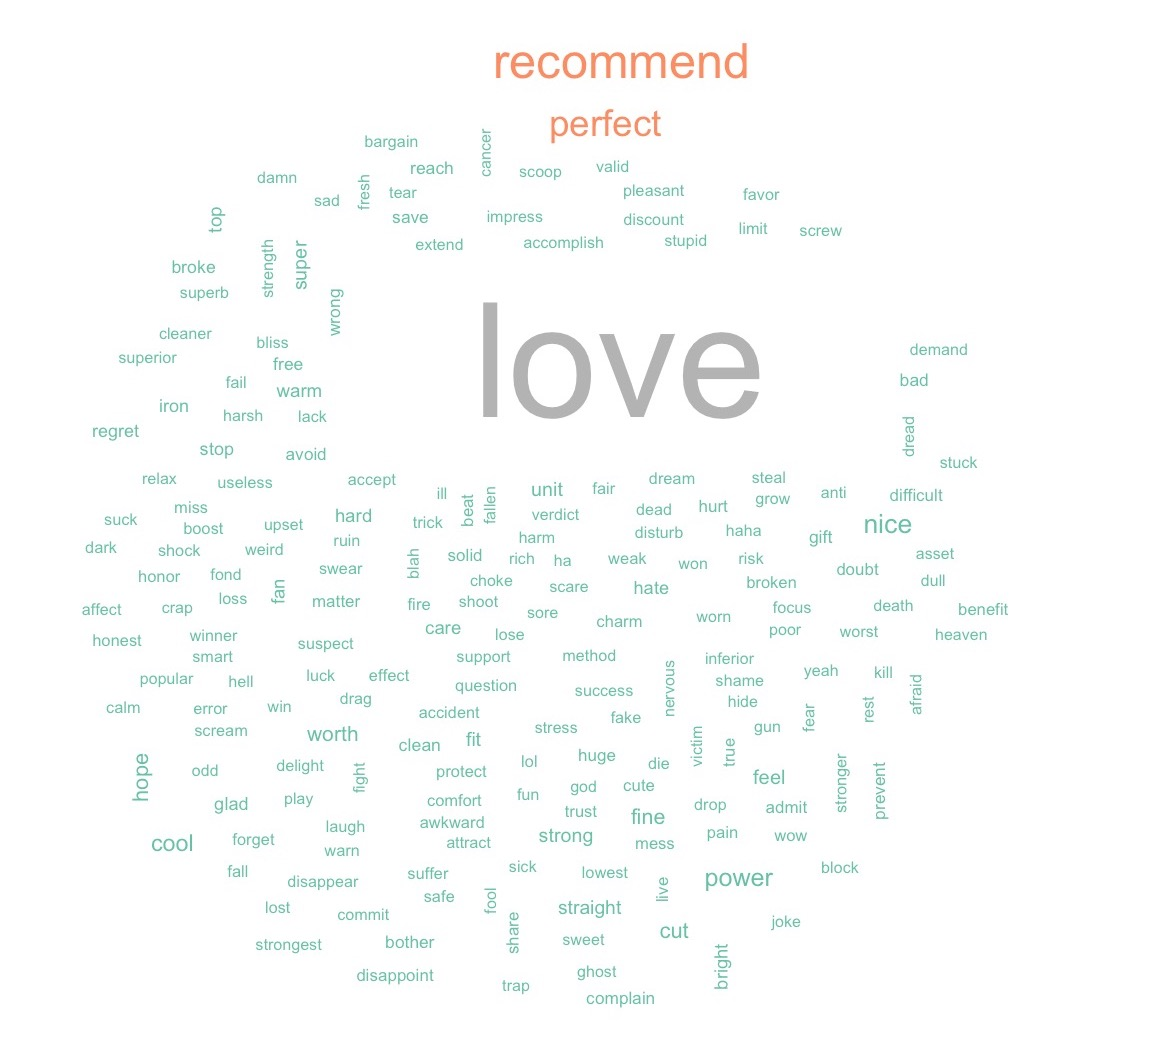
\includegraphics[width=.8\linewidth]{hair45.jpeg}
     \caption{Cloud of high ratings}\label{Fig:4,5}
   \end{minipage}\hfill
   \begin{minipage}{0.48\textwidth}
     \centering
     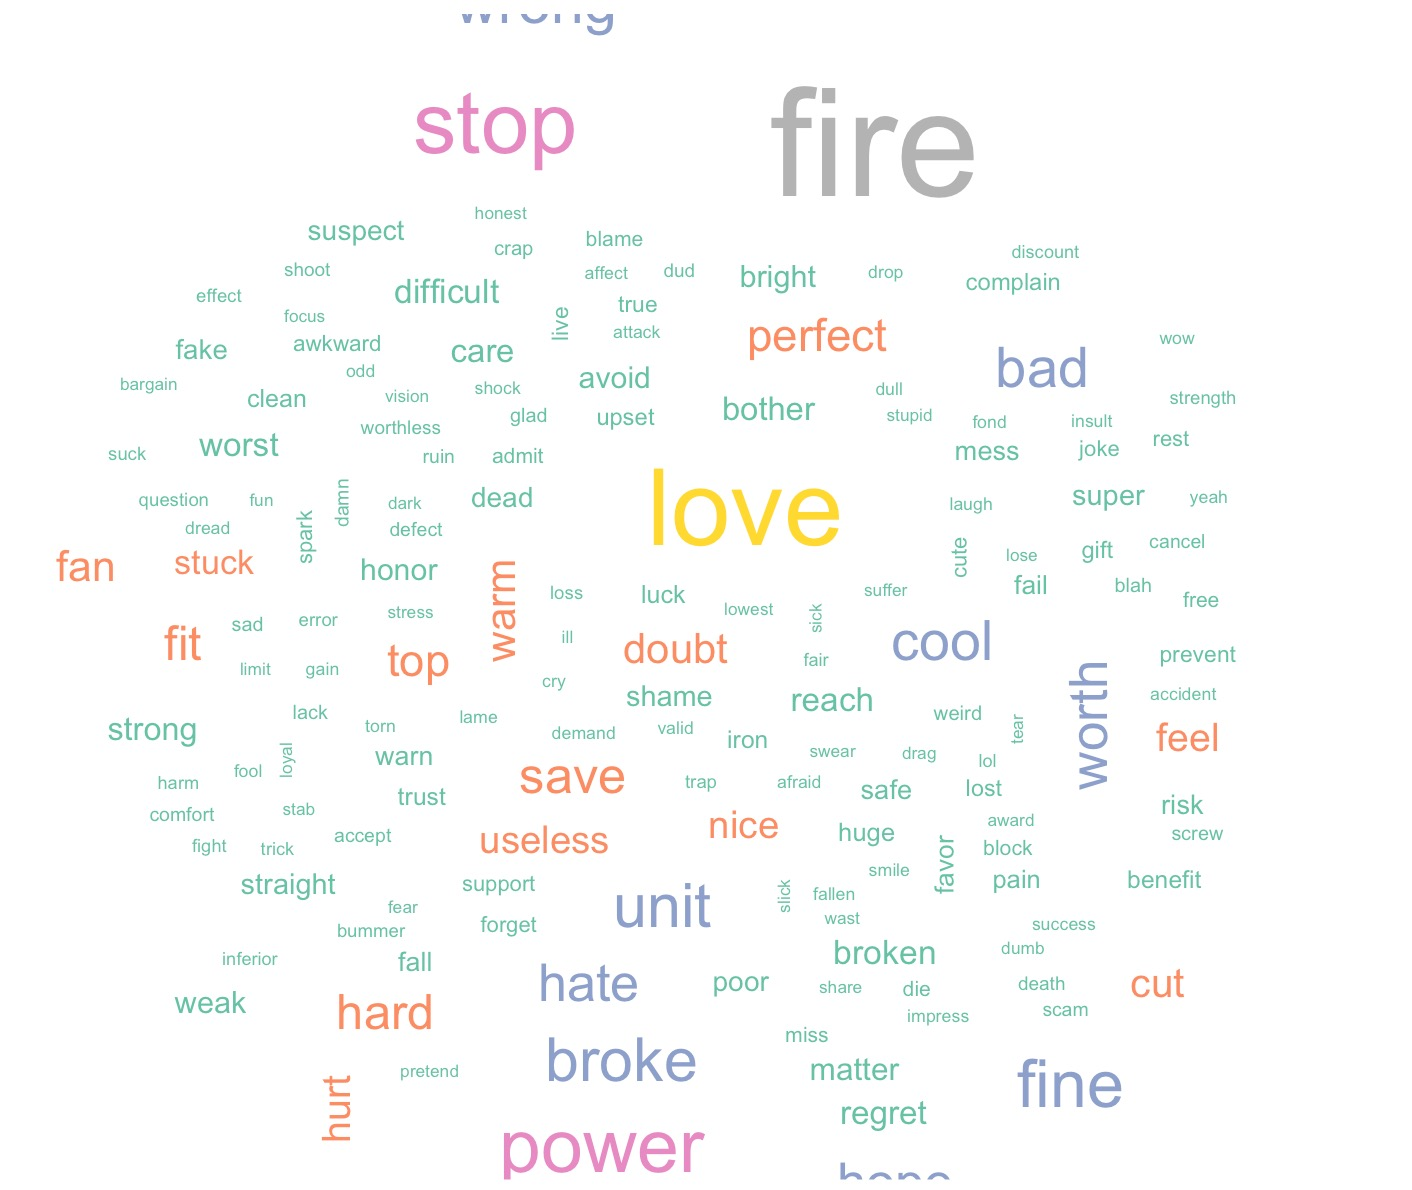
\includegraphics[width=.8\linewidth]{hair12.jpeg}
     \caption{Cloud of low ratings}\label{Fig:1,2}
   \end{minipage}
\end{figure} \\
When it comes to the word count of review text within each rating group, we found that words like 'recommend', 'love' also appears a lot in low rating groups, since they are combined with words like 'not'. Thus, we adopt the Natural Language Processing package in Python to give a sentimental grade to each word, filter out the words with positive rates, and count the appearance of the rest in low rating group.

\begin{table}[!htb]
    \begin{minipage}{.5\linewidth}
      \centering
        \begin{tabular}{ll}
        \hline
            Word & Count \\
            \hline
            love & 10915\\
            \hline
            recommend & 2481\\
            \hline
            perfect & 1584\\
            \hline
            nice & 809\\
            \hline
            power & 703\\
            \hline
        \end{tabular}
        \caption{Word count of high ratings}
    \end{minipage}%
    \begin{minipage}{.5\linewidth}
      \centering
               \begin{tabular}{ll}
        \hline
            Word & Count \\
            \hline
            fire & 312\\
            \hline
            stop & 164\\
            \hline
            power & 137\\
            \hline
            unit & 106\\
            \hline
            support & 91\\
            \hline
        \end{tabular}
        \caption{Word count of low ratings}
    \end{minipage} 
\end{table}

From the Word Cloud and Tables, we can see that in positive ratings, words like 'love' and 'recommend' appear the most, which indicates customers tend to promote the product if they find it satisfactory. Words like 'power' also has large number of appearance, which indicates the power of hair dryer plays a large role in customers' preference. In negative ratings, the most frequent words indicates common problems within the functions of hairdryer. The detailed result will be discussed in the Result section.

\subsubsection{Microwave Review Analysis}
We then adopt the same method to Microwave products:
\begin{figure}[!htb]
   \begin{minipage}{0.48\textwidth}
     \centering
     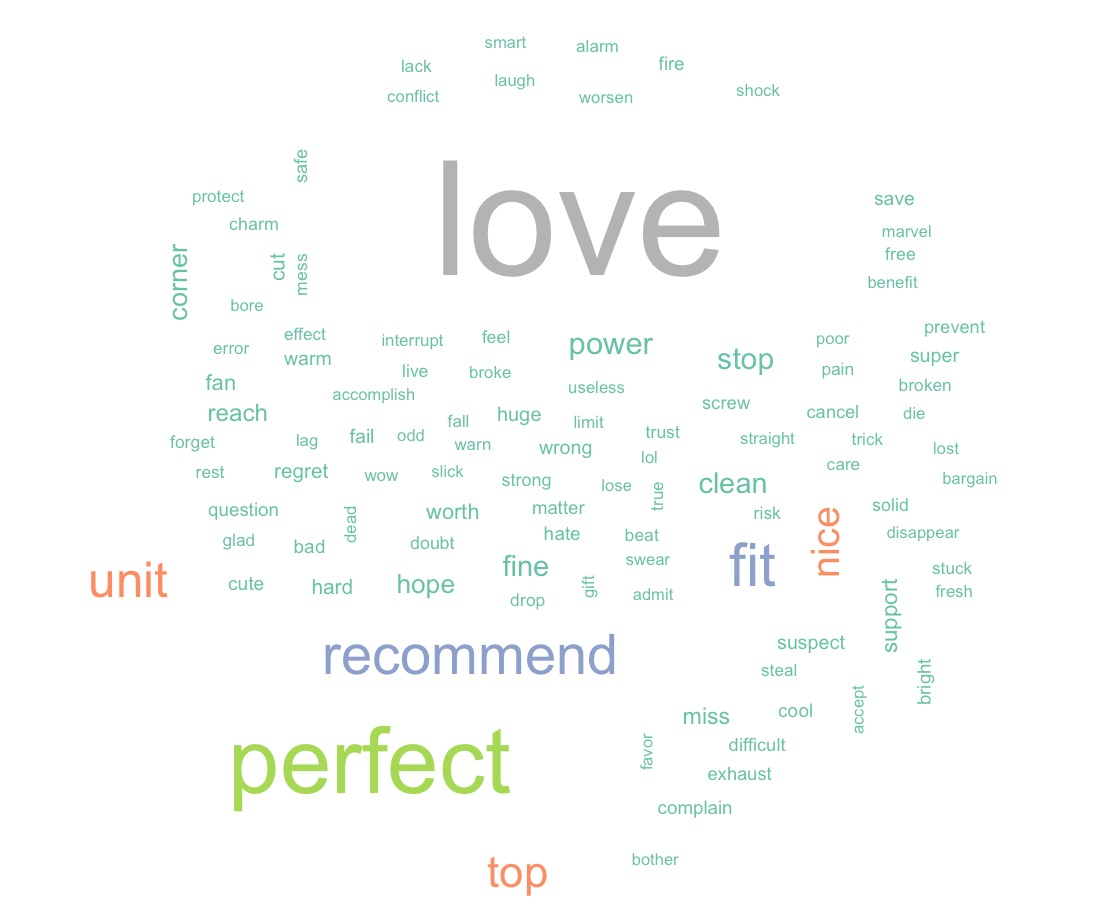
\includegraphics[width=.8\linewidth]{micro45.jpeg}
     \caption{Cloud of high ratings}\label{Fig:4,5}
   \end{minipage}\hfill
   \begin{minipage}{0.48\textwidth}
     \centering
     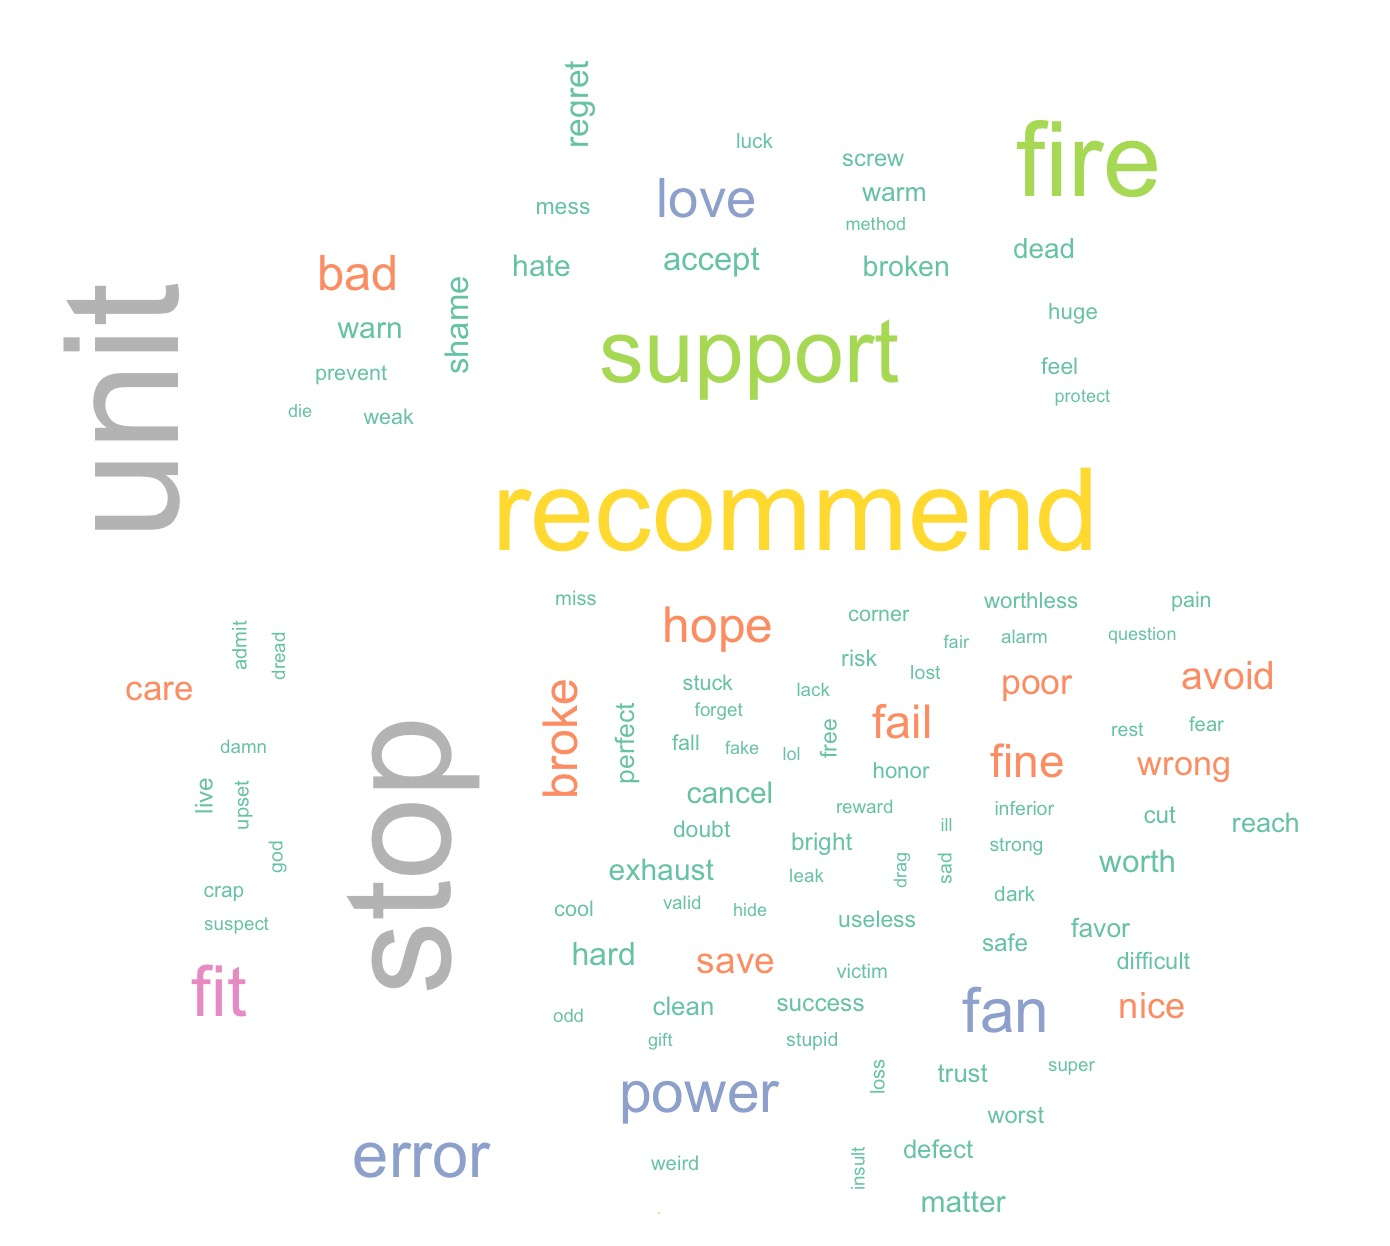
\includegraphics[width=.8\linewidth]{micro12.jpeg}
     \caption{Cloud of low ratings}\label{Fig:1,2}
   \end{minipage}
\end{figure} \\
The following is the word count in high rating group and low rating group:

\begin{table}[!htb]
    \begin{minipage}{.5\linewidth}
      \centering
        \begin{tabular}{ll}
        \hline
            Word & Count \\
            \hline
            love & 775\\
            \hline
            perfect & 411\\
            \hline
            fit & 238\\
            \hline
            recommend & 216\\
            \hline
            unit & 181\\
            \hline
        \end{tabular}
        \caption{Word count of high ratings}
    \end{minipage}%
    \begin{minipage}{.5\linewidth}
      \centering
               \begin{tabular}{ll}
        \hline
            Word & Count \\
            \hline
            unit & 205\\
            \hline
            stop & 188\\
            \hline
            fire & 126\\
            \hline
            top & 120\\
            \hline
            support & 105\\
            \hline
        \end{tabular}
        \caption{Word count of low ratings}
    \end{minipage} 
\end{table}
From the above result, we can see that, except for words like 'love' and 'perfect', words like 'fit' also indicates customers' preference point toward microwave product. In negative rating group, 'stop', 'fire', 'support' indicates common problems of existing microwave products. 

\subsubsection{Pacifier Review Analysis}
Finally adopt the same method to product of pacifier:
\begin{figure}[!htb]
   \begin{minipage}{0.48\textwidth}
     \centering
     
\includegraphics[width=.8\linewidth]{paci45.jpeg}
     \caption{Cloud of high ratings}\label{Fig:4,5}
   \end{minipage}\hfill
   \begin{minipage}{0.48\textwidth}
     \centering
     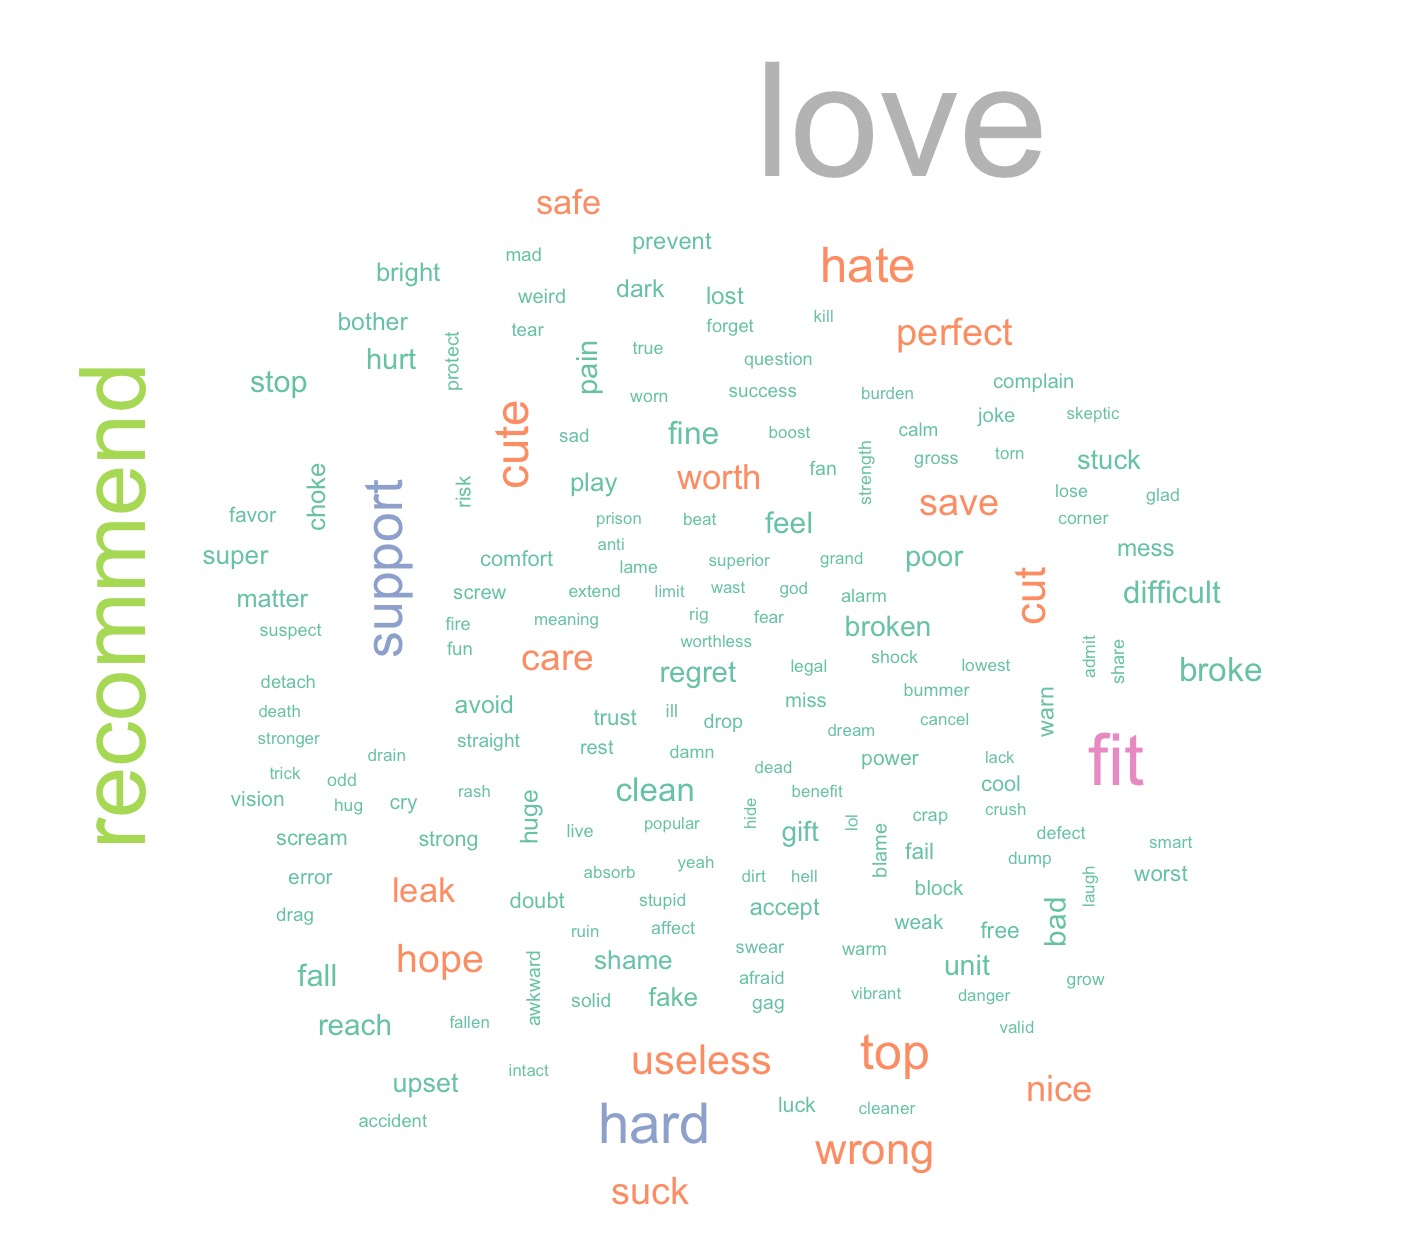
\includegraphics[width=.8\linewidth]{paci12.jpeg}
     \caption{Cloud of low ratings}\label{Fig:1,2}
   \end{minipage}
\end{figure} 

The following is the word count in high rating group and low rating group:
\begin{table}[!htb]
    \begin{minipage}{.5\linewidth}
      \centering
        \begin{tabular}{ll}
        \hline
            Word & Count \\
            \hline
            love & 17730\\
            \hline
            recommend & 3168\\
            \hline
            cute & 1680\\
            \hline
            fit & 1256\\
            \hline
            nice & 1009\\
            \hline
        \end{tabular}
        \caption{Word count of high ratings}
    \end{minipage}%
    \begin{minipage}{.5\linewidth}
      \centering
               \begin{tabular}{ll}
        \hline
            Word & Count \\
            \hline
            fit & 230\\
            \hline
            hard & 166\\
            \hline
            support & 154\\
            \hline
            hate & 136\\
            \hline
            cut & 114\\
            \hline
        \end{tabular}
        \caption{Word count of low ratings}
    \end{minipage} 
\end{table}
From the above analysis, in high rating group, apart from common words like 'love', 'cute', 'fit', 'nice' also have a large number of appearance, indicates customer pay attention to these features when they judge a product of pacifier. In low rating group, words with most appearance also shows problems pacifier may have, which Sunshine Company should try to avoid. 

\subsection{Relationship Within Review Factors}
In this section, we analyze the relationship between the review factors, to see whether the change of one sector will result in customers' differnt review reactions. We calculate the correlation coefficient between some attributes of the product data set by:
\[r_{xy}=\frac{\sum_{i=1}^{n}\left(x_{i}-\bar{x}\right)\left(y_{i}-\bar{y}\right)}{\sqrt{\sum_{i=1}^{n}\left(x_{i}-\bar{x}\right)^{2}} \sqrt{\sum_{i=1}^{n}\left(y_{i}-\bar{y}\right)^{2}}}\]
where $r_{xy}$ is the correlation between attribute $x$ and attribute $y$. The attributes we take into consideration are: the length of review body(denoted as Word count); the number of vine users; the number of verified records; the proportion of helpful votes; the star ratings; and the proportion of high ratings among all the reviews(denoted as good ratio). The data are processed at at daily base. 

\begin{figure}[h]
\caption{Correlation between attributes of hair dryer data}
\centering
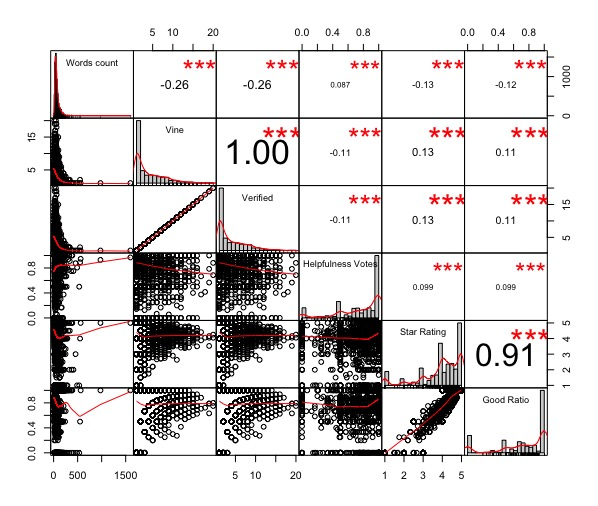
\includegraphics[width=0.45\textwidth]{hairCorr1.jpeg}
\end{figure}
From Figure.7, in the market of hair dryer, we can see the length of review text have negative relationship with all attributes except helpfulness of votes. This indicates customers tend to write longer reviews for low-rating products, and there is fewer vine customers and verified purchases. Number of vine customers have a linear relationship, they both have positive correlation with star rating and good ratio. Helpful votes also have positive relationship with star rating and good ratio, while it has a slightly negative relationship with number of vine customers and verified purchases. One thing worth noticing is that, in hair dryer market, star rating and good ratio have nearly linear relationship.

\begin{figure}[h]
\caption{Correlation between attributes of microwave data}
\centering
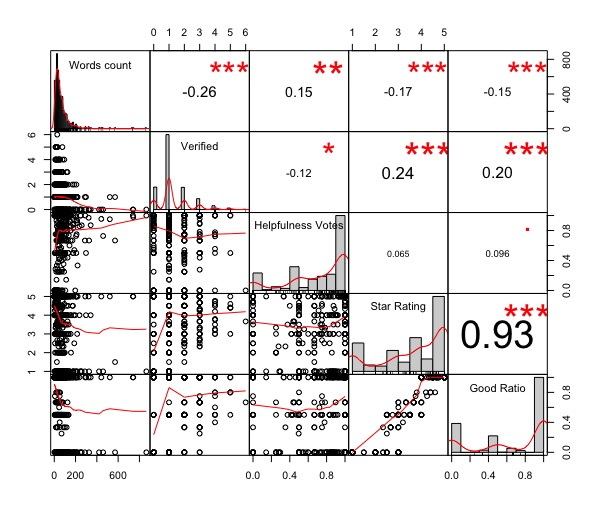
\includegraphics[width=0.45\textwidth]{mcorrelation1.jpeg}
\end{figure}
From Figure.8 generated by data from microwave product, correlations are similar from that within the hair dryer. The length of review body still maintain negative relationship with all attributes except helpfulness of vote. Helpful votes has positive relationship with star rating and good ratio while have negative relationship with number of verified purchase. Star rating and good ratio still maintain a nearly linear correlation in market of microwave products.

\begin{figure}[h]
\caption{Correlation between attributes of pacifier data}
\centering
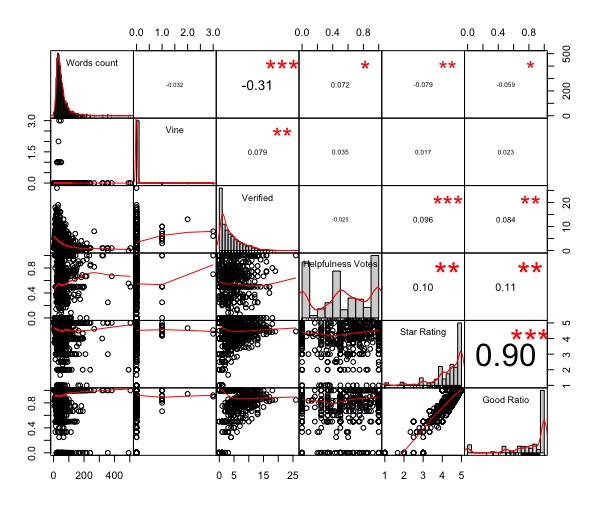
\includegraphics[width=0.45\textwidth]{pcorrelation1.jpeg}
\end{figure}
Similar plot Figure.9 is generated for pacifier's data. In this case, the number of vine customers and verified purchases only have weak correlation. Helpful votes have positive relationship with number of vine customers while have weak negative correlation with number of verified purchases. Except for length of review body, all the other attributes remain positive correlation with star rating and good ratio. Star rating and good ratio keep maintaining a strong positive correlation in market of pacifier.

Based on the correlation analysis of the market data of these three products, some common conclusions can be drawn: Low product ratings often incite reviewers to write longer comments, which includes the problems of the product, while reviews with high ratings tend to short, and longer reviews tend to be more helpful; Products with more verified purchases, vine customers, tend to have higher star rating; In the three product cases, star rating and good ratio all have a strong correlation which is almost linear, thus, in the following section of constructing time series model, we define good ratio as the indicator of the products' selling situation.

\newpage
\subsection{Time Series of Model of Rating and Good Ratio}
Recurrent Neural Network (RNN) has exhibited the power on analyzing time series data prediction. Each node at a time step takes an input from previous node and this can be indicated using a feedback loop.

Even though RNN indicates a strong ability to analyze the correlation in time series data, it has disadvantages in solving long term time series data, which means to understand the context at time step $t+1$, it may require information representing at time $0$ and $1$. To capturer the high dependency in time series,the Long Short Term Memory(LSTM) is invented by Hochreiter and Schmidhuber\cite{Hlstm}. Based on typical RNN structure, each cell is indicated by a more complex inner network with the crucial components, gates. Comparing with a single neural layer in RNN, there are four interacting gates, input gate, forget gate, update gate, and output gate. The gated structure, especially crucial forget gate and the update gate, supports LSTM to remember information in the long term time series optionally, and decides vital information to update to the cell state. It has proved that the bidirectional networks \cite{BiLSTM} are sincerely better than the traditional LSTM in many fields capturing time-series information. 

In this work, we define stacked bidirectional LSTM with two layers as the first temporal features or information abstraction, then connect with one layer LSTM to remedy potential temporal correlation. After stacked BiLSTM and LSTM, two Dense layers added at the end, which is capable of reasonably controlling dimensions in hidden layers output, and more precisely capture nonlinearity between inputs and outputs since inputs in our model are multivariate with abstract correlations.            

In this study, we use features $R_{G}$, $P_{v}$, $n_{word}$, $n_{veri}$ and $n_{vine}$ to predict $R_{S}$ since there exists correlation among Average star rating and other factors. Similarly, we also use features $R_{S}$, $P_{v}$, $n_{word}$, $n_{veri}$ and $n_{vine}$ to predict $R_{G}$. Each data point represents the daily average on day t. For example, when we predict the average daily good ratio of pacifier on day t, $R_{G}$, we use features from two historical time steps(two days), t−2 to t − 1, to predict. The input can be characterized as an input features matrix:
\begin{equation*}
X_{t} =\begin{bmatrix}
\textit{$R_{G,t-2}$}&\textit{$R_{S,t-2}$}&\textit{$N_{word,t-2}$}&\textit{$N_{veri,t-2}$}&\textit{$N_{vine,t-2}$}&\textit{$P_{v,t-2}$} \\

&&&&&\\
\textit{$R_{G,t-1}$}&\textit{$R_{S,t-1}$}&\textit{$N_{word,t-1}$}&\textit{$N_{veri,t-1}$}&\textit{$N_{vine,t-1}$}&\textit{$P_{v,t-1}$}

\end{bmatrix}
\end{equation*}
where 
\begin{itemize}
 \item \textit{$R_{S,t-2}$} = Average daily star rating at historical time segment \textit{$t-2$} 
 \item \textit{$N_{word,t-2}$} = Average daily words count at historical time segment \textit{$t-2$} 
 \item $P_{v,t-2}$ = Average daily helpfulness votes at historical time segment \textit{$t-2$}
\end{itemize} 
Similar meanings for all other notations in the input matrix $X_{t}$.

\subsection{Test of Model Accuracy}
Final prediction results using evaluation metrics RMSE, which is defined as follows:
\begin{equation}
    RMSE = \sqrt{\frac{1}{n}\sum_{i = 1}^{n}(\hat{y_{i}} - y_{i})^{2}}
\label{RMSE}
\end{equation}
where $\hat{y_i}$ is a predicted value, $y_i$ is the corresponding true value and $n$ is the number of predicted values.

\subsubsection{Hair Dryer}

\begin{figure}[!htb]
   \begin{minipage}{0.48\textwidth}
     \centering
     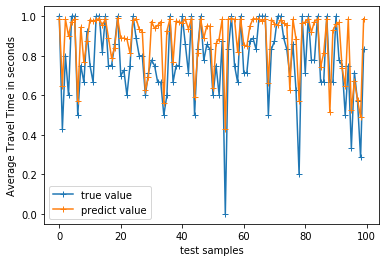
\includegraphics[width=.8\linewidth]{hairratio_RMSE0131.png} % RMSE0131
     \caption{Hairdryer Average Good Ratio Predtion}\label{hairgr}
   \end{minipage}\hfill
   \begin{minipage}{0.48\textwidth}
     \centering
     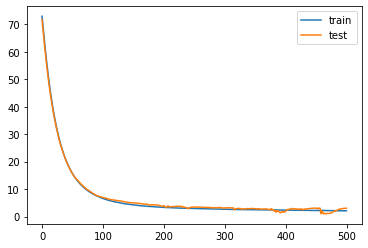
\includegraphics[width=.8\linewidth]{microloss.png}
     \caption{Loss Function of Hairdryer Average Good Ratio Predtion}\label{hairgrloss}
   \end{minipage}
\end{figure} 

\begin{figure}[!htb]
   \begin{minipage}{0.48\textwidth}
     \centering
     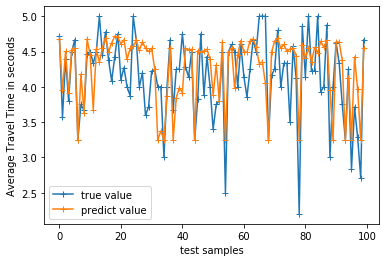
\includegraphics[width=.8\linewidth]{rate_RMSE0528.png} %RMSE0528
     \caption{Hair Dryer Average Star Rating Predtion}\label{hairsr}
   \end{minipage}\hfill
   \begin{minipage}{0.48\textwidth}
     \centering
     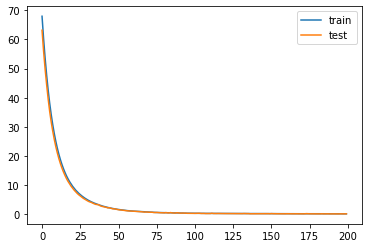
\includegraphics[width=.8\linewidth]{loss.png}
     \caption{Loss Function of Hairdryer Average Star Rating}\label{hairsrloss}
   \end{minipage}
\end{figure} 

Figure(\ref{hairgr}-\ref{hairsr}) shows the results of the prediction of the average daily good ratio $R_{G}$ at time t and the prediction of the average daily star rating $R_{S}$ at time t, respectively. Figure(\ref{hairgrloss}-\ref{hairsrloss}) shows the loss function of training and testing. The RMSE, which is defined in Equation(\ref{RMSE}), of predicting $R_{G}$ at time t is 0.131 and of predicting $R_{S}$ at time t is 0.528. 

\subsubsection{Microwave}

\begin{figure}[!htb]
   \begin{minipage}{0.48\textwidth}
     \centering
     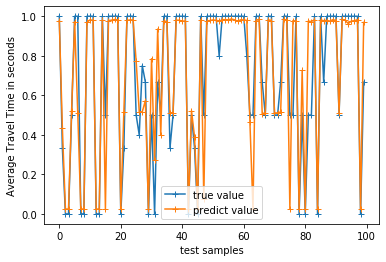
\includegraphics[width=.8\linewidth]{mratio_prediction_RMSE0177.png} %RMSE0177
     \caption{Microwave Average Good Ratio Predtion}\label{microgr}
   \end{minipage}\hfill
   \begin{minipage}{0.48\textwidth}
     \centering
     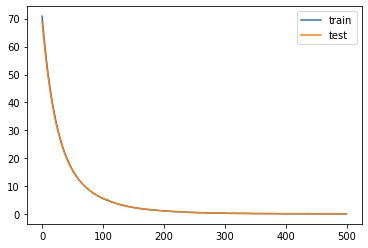
\includegraphics[width=.8\linewidth]{mratio_loss.png}
     \caption{Loss Function of Microwave Average Good Ratio}\label{microgrloss}
   \end{minipage}
\end{figure} 


\begin{figure}[!htb]
   \begin{minipage}{0.48\textwidth}
     \centering
     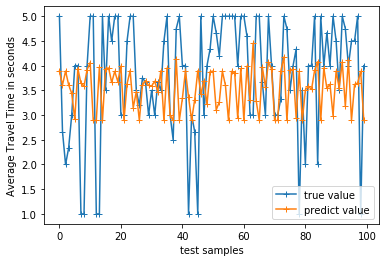
\includegraphics[width=.8\linewidth]{micro_prediction1211.png} %RMSE1211 
     \caption{Microwave Average Star Rating Predtion}\label{microsr}
   \end{minipage}\hfill
   \begin{minipage}{0.48\textwidth}
     \centering
     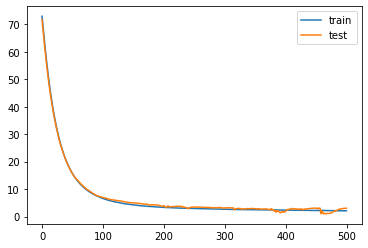
\includegraphics[width=.8\linewidth]{microloss.png}
     \caption{Loss Function of Microwave Average Star Rating}\label{microsrloss}
   \end{minipage}
\end{figure} 

Figure(\ref{microgr}-\ref{microsr}) shows the results of the prediction of the average daily good ratio $R_{G}$ at time t and the prediction of the average daily star rating $R_{S}$ at time t, respectively. Figure(\ref{microgrloss}-\ref{microsrloss}) shows the loss function of training and testing. The RMSE, which is defined in Equation(\ref{RMSE}), of predicting $R_{G}$ at time t is 0.177 and of predicting $R_{S}$ at time t is 1.211. 

\subsubsection{Pacifier}

\begin{figure}[!htb]
   \begin{minipage}{0.48\textwidth}
     \centering
     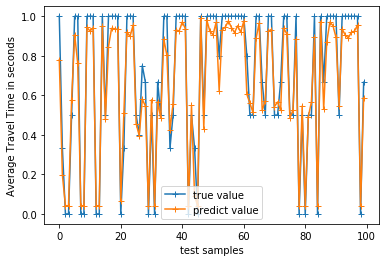
\includegraphics[width=.8\linewidth]{pacifier_ratio_0095.png} %RMSE0095
     \caption{Pacifier Average Good Ratio Predtion}\label{pacigr}
   \end{minipage}\hfill
   \begin{minipage}{0.48\textwidth}
     \centering
     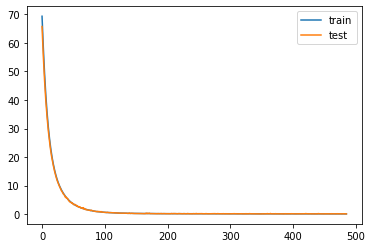
\includegraphics[width=.8\linewidth]{pacifier_ratio_loss.png}
     \caption{Loss Function of Pacifier Average Good Ratio}\label{pacigrloss}
   \end{minipage}
\end{figure} 


\begin{figure}[!htb]
   \begin{minipage}{0.48\textwidth}
     \centering
     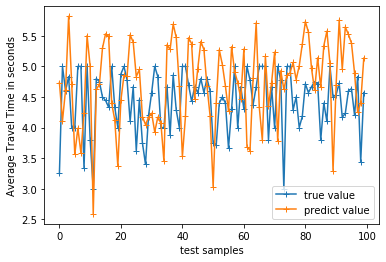
\includegraphics[width=.8\linewidth]{pacifer_prediction_0935.png} %RMSE0935
     \caption{Pacifier Average Star Rating Predtion}\label{pacisr}
   \end{minipage}\hfill
   \begin{minipage}{0.48\textwidth}
     \centering
     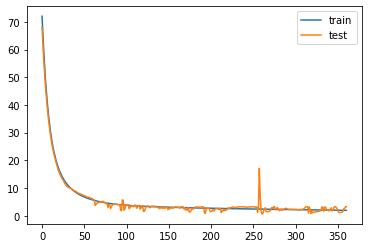
\includegraphics[width=.8\linewidth]{pacifier_loss.png}
     \caption{Loss Function of Pacifier Average Star Rating}\label{pacisrloss}
   \end{minipage}
\end{figure} 

Figure(\ref{pacigr}-\ref{pacisr}) shows the results of the prediction of average daily good ratio $R_{G}$ at time t and the prediction of average daily star rating $R_{S}$ at time t, respectively. Figure(\ref{pacigrloss}-\ref{pacisrloss}) shows the loss function of training and testing. The RMSE, which is defined in Equation(\ref{RMSE}), of predicting $R_{G}$ at time t is 0.095 and of predicting $R_{S}$ at time t is 0.935. 

\subsubsection{Conclusion of the Time Series Model}
From the results of the prediction of the average daily good ratio $R_{G}$ at time t and the prediction of the average daily star rating $R_{S}$ at time t, we could conclude that the good ratio, which depicts the trend of a customer to give a product a high star rate, could be well predicted using the information of the previous two time segments using our proposed Multi-Stacked Fully Connected Bidirectional LSTM model(MSFCB-LSTM). Nevertheless, we could use our proposed model to predict the star rate at time t, the results of the prediction are not all accurate due to the reasons that the deficiency of information. But the patterns of changes of star rating could be well described. Thus, we could combine the results of the prediction of average daily good ratio $R_{G}$ at time t and average daily star rating $R_{S}$ at time t together to make decisions.

\section{Results}


\subsection{Identification of Crucial Product Features}
In this section, we will analyze what Sunshine Company should focus on improving their upcoming product, based on the previous text mining results. Apart from filtering out the most common words within each range of rating, we also referred to the complete text of review records containing these words.
\subsubsection{Hair Dryer}
Among positive ratings, besides common phrasing words, word count shows that customers favor most about the machines' power when they give good ratings. Sunshine company should also keep high quality of machines' power, since many other brands are doing good. 

Among negative ratings, we first go through complete review texts of frequent words which have positive sentimental grade(Given by NLP method). By going through reviews containing word 'recommend', in which customers expressed they wouldn't recommend, problems with other hair dryer includes short battery life, coming out cold air, and loud noise. Among negative reviews containing 'unit', customers complained about the short life of the product, poor quality of material, insufficient power, and bad design. 

Combine these results with word 'fire', 'power', 'stop', we can see that in existing market, the common problems with hair dryer such as : battery life, inappropriate temperature, loud noise, short lifespan, bad design, are the points Sunshine Company should focus on improving their current product before putting them to the market and thus increase its competence. 

\subsubsection{Microwave}
Among positive ratings, apart from common words like 'love', the frequent appearance of 'fit' indicates the size of microwave product plays a important role in customers' preference.

Among negative ratings, we go through the complete review record of words which have positive sentimental grade. In text containing 'recommend', customers don't recommend a product due to inappropriate size, bad function, short lifespan. Complains including word 'unit' mainly due to customer support, bad function, power problems.

Combining the above analysis with other frequent words 'stop', 'fire', we can conclude that Sunshine Company should focus on improving its' microwave product's heating function, design more appropriate size by doing more customer survey, also pay more attention to improve customer service, and thus increase competence in existing market.

\subsubsection{Pacifier}
Among the positive ratings of pacifiers, we can see that 'cute' and 'fit' indicate customers pay more attention to pacifiers' appearance and size when judging. Thus Sunshine Company should keep the appearance of their product cute and design pacifiers with appropriate size to keep competence. 

Among negative ratings' records, we first analyze frequent words with positive NLP grade. Based on complete review text, customers don't recommend products due to: making loud noise, useless to keep babies quiet, bad material, and bad function. Bad reviews containing 'support' mostly due to no customer service support, product doesn't work well with other devices.

Combining the results above and other words appear frequently in negative reviews: 'hard', 'fit', we can conclude that, to compete with existing pacifier products, Sunshine Company should focus on improving the pacifiers' function, material, reducing the noise, and improve its size design to fit with the other corresponding devices like bottles. 


\subsection{Indicators for Sales Tracking}
Some researchers have revealed that customers are more willing to buy a product that with good ratings. In this study, we use two indicators to represent whether a product is popular and will be sold well. The first indicator is the average daily star ratings, $R_{S_{t}}$. The second indicator is the average daily good ratio, $R_{G_{t}}$, which describes whether a customer would like to give a good star rating. 

To predict the two indicators above, five more features are used:
\begin{itemize}
    \item $N_{vine_{t}}$: Average number of vine customers on time t
    \item $N_{veri_{t}}$: Average number of verified purchase on time t
    \item $N_{word_{t}}$: Average number of words count in the review body on time t.
    \item $P_{v_{t}}$: Average proportion of helpful votes on time t.
\end{itemize}

Besides, we also use NLP to dig the words with high priority, find the sentences with those words to see what disadvantages a product owns. We could summary those negative reviews to improve our products.

\section{Strength and Weakness}
\subsection{Strengths}
\begin{itemize}
    \item We applied various data visualization techniques including word cloud and combined image of correlation to demonstrate the word count distribution intuitively.
    \item We took multiple factors into consideration when constructing the time series model and ...
    \item We adopt method of natural language processing to identify the words expressing customer feelings, and explored the full text consisting these words to draw conclusion.
    \item Our model has high level of accuracy at predicting the future proportion of positive ratings among total reviews.
\end{itemize}

\subsection{Weakness}
\begin{itemize}
    \item For time series analysis, took average of data of all products within each date, more product related factors should be considered in future research.
    \item Made an assumption of ignoring market size factor, which has an effect on product's future success.
    \item In text analysis, we only considered words with top five occurrence, some information might be lost. 
\end{itemize}
\newpage
\section{Letter to Market Director of Sunshine Company}
Date: March 8, 2020\\[0.5ex]
To: Market Director of Sunshine Company\\[0.5ex]
From: MCM Team \# 2018915\\[0.5ex]
Subject: Market Analysis and Strategy Recommendation\\[1.5ex]
Dear Director,
\vskip 0.1in
Hope you are doing well. After conducting a through analysis of the Amazon data of the three type of product Sunshine Company is going to release. Due to the large amount of available products, the current online market has quite intensive competitions. We are writing to provide some advice Sunshine Company might find useful. 
\vskip 0.1in
We analyzed the words, sentiments in customers review text and come up with following suggestions for pre-release stage of products.
\begin{itemize}
    \item For hair dryer, according to customers' review, to compete with other similar products, Sunshine may consider to enhance in products' material quality, power capacity, longer lifespan. Also the noise the machine made and appropriate temperature are also concerns of customers;
    \item For microwave oven, customers pay more attention to the machines' heat function, size, and power capacity. Sunshine may also need to focus on improving customer support for this kind of electronic appliance; 
    \item For pacifier, Sunshine can put more attention on the material, size, and also finding ways to reduce noise will be a good strategy to improve competence. Designing cute products will also help since it's for babies. 
\end{itemize}

After the products are released, it might be useful to track some factors and predict future selling. According to our analysis, having more vine customers and verified purchase, encouraging helpful votes for existing reviews will bring positive effect to the success of the product. Also, it may be a good idea to pay more attention to long reviews, since they possibly contain more information to help improve the product. 
\vskip 0.1in
We understand that releasing new products into market is a very long and complicated process. We believe Sunshine Company has made sufficient preparation for the moment.Due to lack of data, we ignored some challenges in real market, we also didn't put enough weight on analyzing specific products. There will be some information missing in our advice. Doing more customer survey as time goes by is a more sufficient way to keep track of customer opinions. But we sincerely hope our advice can help. We will try to provide more sufficient and accurate information in future cooperation. 
\vskip 0.2in
Best Regards,
\vskip 0.2in
MCM Team 2018915

03/09/2020


% Reference %%%%%
\newpage
\begin{thebibliography}{14}
	\bibitem{maddah2014fundamental}
	M. A. Maddah-Ali, and U. Niesen,  ``Fundamental Limits of Caching", in \emph{IEEE Trans. Inform. Theory}, vol. 60, no. 5, pp. 2856-2867, May 2014.
	\bibitem{Hlstm}S. Hochreiter and J. Schmidhuber, “Long Short-Term Memory,” Neural Computation, vol. 9, no. 8, pp. 1735–1780, 1997.
    \bibitem{BiLSTM} M. Schuster and K. Paliwal, “Bidirectional recurrent neural networks,” IEEE Transactions on Signal Processing, vol. 45, no. 11, pp. 2673–2681, 1997.
\end{thebibliography}
\pagebreak


% appendices %%%%%%%%%%%%%%%%%%%%%%%%%%%%%%%%%%%%%%%%%%%%%%%%%%%%%%%%

\begin{appendices}
\section{Appendices}
\subsection{Code (R)}

\definecolor{dkgreen}{rgb}{0,0.6,0}
\definecolor{gray}{rgb}{0.5,0.5,0.5}
\definecolor{mauve}{rgb}{0.58,0,0.82}
\lstset{frame=tb,
  language=R,
  aboveskip=3mm,
  belowskip=3mm,
  showstringspaces=false,
  columns=flexible,
  basicstyle={\small\ttfamily},
  numbers=none,
  numberstyle=\tiny\color{gray},
  keywordstyle=\color{blue},
  commentstyle=\color{dkgreen},
  stringstyle=\color{mauve},
  breaklines=true,
  breakatwhitespace=true,
  tabsize=3
}
\begin{lstlisting}

# To plot the correlation plot
Data <- read.csv('hraw.csv')
d = as.data.frame(cbind( Data$Average.of.word_counts,
                         Data$Count.of.verified_purchase, Data$Average.of.helpful_rate, 
                         Data$Average.of.star_rating,Data$good_ratio))
colnames(d) <- c('Words count','Verified','Helpfulness Votes','Star Rating','Good Ratio')
cor_matr <- rcorr(as.matrix(d))$r
corrplot(cor_matr, type="upper", order="hclust", tl.col="black", tl.srt=45)
chart.Correlation(d,histogram = TRUE,pch=19)
col = colorRampPalette(c("blue", "white", "red"))(20)

hair_dryer<-as.data.frame(fread('hair_dryer.tsv'))
hair_dryer12 <- hair_dryer[which((hair_dryer$star_rating == 1) | (hair_dryer$star_rating == 2)),]

words <- hair_dryer12 %>%
  select(c("review_id", "star_rating", "review_body")) %>%
  unnest_tokens(word, review_body) %>%
  filter(!word %in% stop_words$word, str_detect(word, "^[a-z']+$"))

afinn <- get_sentiments("afinn") %>% mutate(word = wordStem(word))
reviews.afinn <- words %>%
  inner_join(afinn, by = "word")
head(reviews.afinn)

word_summary <- reviews.afinn %>%
  group_by(word) %>%
  summarise(count_word = n()) %>%
  arrange(desc(count_word))

datatable(head(word_summary))
wordcloud(words = word_summary$word, freq = word_summary$count_word, scale=c(5,.5), max.words=200, colors=brewer.pal(8, "Set2"))
wordrate1 <- word_summary[which(word_summary$count_word >= 50),]
wordrate1 <-cbind(wordrate1$word,wordrate1$count_word)
colnames(wordrate1) <- c('word','count')
write.csv(Data,file="hwordrate1.csv",row.names = F)

\end{lstlisting}

\subsection{Code (Python)}

\definecolor{dkgreen}{rgb}{0,0.6,0}
\definecolor{gray}{rgb}{0.5,0.5,0.5}
\definecolor{mauve}{rgb}{0.58,0,0.82}
\lstset{frame=tb,
  language=Python,
  aboveskip=3mm,
  belowskip=3mm,
  showstringspaces=false,
  columns=flexible,
  basicstyle={\small\ttfamily},
  numbers=none,
  numberstyle=\tiny\color{gray},
  keywordstyle=\color{blue},
  commentstyle=\color{dkgreen},
  stringstyle=\color{mauve},
  breaklines=true,
  breakatwhitespace=true,
  tabsize=3
}

\begin{lstlisting}
# Data Preparation
hair_dryer = pd.read_csv('50.csv')
key = list(hair_dryer.keys())
new = hair_dryer[['marketplace','customer_id','review_id','product_id',
                  'product_parent','product_title','product_category',
                  'star_rating','helpful_vote','total_votes','review_head',
                  'review_body','review_date']]

# To handle with the features
h_body = list(hair_dryer['review_body'])
words_count = []
# Add word counts of the review body
for text in h_body:
    blob = TextBlob(text)
    token = blob.words
    words_count.append(len(token))
words_count = pd.DataFrame(words_count)
vine = list(hair_dryer['vine'])
veri = list(hair_dryer['verified_purchase'])
# Convert Vine and Verified Purchased into numerical
for i in range(len(vine)):
    v = vine[i]
    if v == 'N':
        vine[i] = 0
    else:
        vine[i] = 1
for i in range(len(veri)):
    v = veri[i]
    if v == 'N':
        veri[i] = 0
    else:
        veri[i] = 1
vine = pd.DataFrame(vine)
veri = pd.DataFrame(veri) 
tosave = pd.concat([new,vine,veri,words_count],axis = 1)
tosave.columns = ['marketplace','customer_id','review_id','product_id','product_parent',
                  'product_title','product_category','star_rating','helpful_vote',
                  'total_votes','review_head',
                  'review_body','review_date','vine','veri','word']
tosave.to_csv('hairdryer50.csv')
# To find the Good Ratio and combine them with the original data set
data = pd.read_csv('hairdryer50.csv')
data = data[data.columns[1:]]
date = list(set(data['review_date']))
date_dict = {}
for d in date:
    date_dict[d] = []

info = np.array(data)
for i in range(len(info)):
    rate = info[i][6]
    da = info[i][13]
    date_dict[da].append(rate)

keys = sorted(list(date_dict.keys()))
count = []
for k in keys:
    j = date_dict[k]
    length = len(j)
    c = len([1 for i in j if i >= 4])
    count.append(c/length)
count = pd.DataFrame(count)
hraw = pd.read_csv('hairdryer.csv')
a = pd.concat([hraw,count],axis = 1)
a.columns = ['Date','Average of word_counts','Average of helpful_rate',
              'Count of verified_purchase', 'Count of vine','Average of star_rating','good_ratio']
a.to_csv('hraw.csv')

# Words Grading and Sentences Collection
nltk.download('punkt')
review = pd.read_csv('hrate1.csv')['review_body']
cols = pd.read_csv('hwordrate1.csv').columns
word = pd.read_csv('hwordrate1.csv')[cols[0]]
count = pd.read_csv('hwordrate1.csv')[cols[1]]

# To find the grate of the words that appear more than 50 times in the review body
grade = []
for w in word:
    blob = TextBlob(w)
    for sentence in blob.sentences:
        print(sentence + '------>'+ str(sentence.sentiment.polarity))
        grade.append(sentence.sentiment.polarity)
grade = pd.DataFrame(grade)
a = pd.concat([word,count,grade],axis = 1)
a.columns = ['word','count','grade']
a.to_csv('hwordrate1.csv')

# To find the sentences that contains words with non-positive grade
from textblob import TextBlob
check_word = word[12]
sentence_list = []

for i in range(len(review)):
    text = review[i]
    blob = TextBlob(text)
    for sentence in blob.sentences:
        if check_word in sentence:
            sentence_list.append(str(sentence))
sentence_list = pd.DataFrame(sentence_list)
sentence_list.columns = [check_word]
sentence_list.to_csv('hairdryer_%s.csv'%(check_word))

# MSFCB-LSTM
def series_to_supervised(data, n_in=1, n_out=1, dropnan=True):
    n_vars = 1 if type(data) is list else data.shape[1]
    df = pd.DataFrame(data)
    cols, names = list(), list()
    # input sequence (t-n, ... t-1)
    for i in range(n_in, 0, -1):
        cols.append(df.shift(i))
        names += [('var%d(t-%d)' % (j+1, i)) for j in range(n_vars)]
    # forecast sequence (t, t+1, ... t+n)
    for i in range(0, n_out):
        cols.append(df.shift(-i))
        if i == 0:
            names += [('var%d(t)' % (j+1)) for j in range(n_vars)]
        else:
            names += [('var%d(t+%d)' % (j+1, i)) for j in range(n_vars)]
    # put it all together
    agg = pd.concat(cols, axis=1)
    agg.columns = names
    # drop rows with NaN values
    if dropnan:
        agg.dropna(inplace=True)
    return agg

def Bnorm(model):
    model.add(BatchNormalization(axis=1, momentum=0.99, epsilon=0.001))

def get_lr_metric(optimizer):
    def lr(y_true, y_pred):
        return optimizer.lr
    return lr

dataset = pd.read_csv('praw.csv',index_col = 0)
a = dataset.columns
dataset = dataset[a[1:]]
dataset.columns = ['word','helpful_rate','veri','vine','star_rating','good_ratio']
dataset['word'].fillna(0, inplace=True)
dataset['vine'].fillna(0, inplace=True)
dataset['veri'].fillna(0, inplace=True)
dataset['helpful_rate'].fillna(0, inplace=True)
dataset['star_rating'].fillna(0, inplace=True)
dataset['good_ratio'].fillna(0, inplace=True)
values = dataset.values
# ensure all data is float
values = values.astype('float32')
# normalize features
scaler = MinMaxScaler(feature_range=(0, 1))
scaled = scaler.fit_transform(values)
# frame as supervised learning
reframed = series_to_supervised(values, 1, 1)
# To choose the index of the predictors
var = [0,1,2,3,4,6,7,8]
# split into train and test sets
values = reframed.values
n_obs = int(len(values)*0.7)
train = values[:n_obs, :]
test = values[n_obs:, :]
# split into input and outputs
train_X, train_y = train[:, var], train[:, -1]
test_X, test_y = test[:, var], test[:, -1]
# reshape input to be 3D [samples, timesteps, features]
train_X = train_X.reshape((train_X.shape[0], 1, train_X.shape[1]))
test_X = test_X.reshape((test_X.shape[0], 1, test_X.shape[1]))
print(train_X.shape, train_y.shape, test_X.shape, test_y.shape)

# set GPU
os.environ["CUDA_VISIBLE_DEVICES"]="1"
config = tf.ConfigProto()
# config.gpu_options.per_process_gpu_memory_fraction = 0.6 
session = tf.Session(config=config)
KTF.set_session(session )

lr = 0.001
masking_func = lambda inputs, previous_mask: previous_mask[:, N:]
# Batch_Size=1
model = Sequential()
model.add(Bidirectional(LSTM(50,return_sequences=True,
                             input_shape=(train_X.shape[1],train_X.shape[2]),
                             kernel_initializer='he_normal',
                             #kernel_regularizer=regularizers.l2(0.05)
                             dropout=0.02,recurrent_dropout = 0.02,
                             kernel_regularizer=regularizers.l2(0.03))))
Bnorm(model)

model.add(Dense(output_dim=100,activation= 'relu'))##
Bnorm(model)

model.add(Bidirectional(LSTM(50,return_sequences=True,
                             kernel_initializer='he_normal',
                             #kernel_regularizer=regularizers.l2(0.05)
                             dropout=0.02,recurrent_dropout = 0.02,
                            kernel_regularizer=regularizers.l2(0.03))))                           
Bnorm(model)


model.add(Bidirectional(LSTM(30,return_sequences=True,
                            kernel_initializer='he_normal',
                             #kernel_regularizer=regularizers.l2(0.05)
                             dropout=0.02,recurrent_dropout = 0.02,
                            kernel_regularizer=regularizers.l2(0.03))))                           
Bnorm(model)
model.add(Dense(output_dim=50,activation= 'relu'))##
Bnorm(model)
model.add(LSTM(50, return_sequences=False,kernel_initializer='he_normal',
               dropout=0.01,recurrent_dropout = 0.01,
                kernel_regularizer=regularizers.l2(0.02)))
Bnorm(model)
model.add(Dense(output_dim=100, activation= 'relu'))
Bnorm(model)
model.add(Dense(output_dim=100,activation = 'relu'))
Bnorm(model)
model.add(Dense(output_dim=100,activation = 'relu'))
Bnorm(model)
model.add(Dense(output_dim=1))
model.add(Activation('relu'))
Bnorm(model)

adam=Adam(lr,decay=0.0005)
model.compile(loss='mae', optimizer=adam)
from keras.callbacks import EarlyStopping
 
early_stopping=EarlyStopping(monitor='val_loss', min_delta=0,
                              patience=100, verbose=0, mode='auto',
                              baseline = None, restore_best_weights = True)

history = model.fit(train_X, train_y, epochs=500, ##
                    batch_size=80, validation_split=0.05, shuffle=False,
                    callbacks=[early_stopping])
    
#### Test Ratio  with word count
pyplot.plot(history.history['loss'], label='train')
pyplot.plot(history.history['val_loss'], label='test')
pyplot.legend()
pyplot.show()
plt.figure()
yhat = model.predict(test_X)
test_y = test_y.reshape((len(test_y), 1))
# To print the first 100 predictions in the test data set.
plt.plot([x for x in range(len(test_y[0:100])) ],test_y[0:100],[x for x in range(len(test_y[0:100])) ],yhat[0:100],marker='+', linestyle='-')
plt.xlabel('test samples')
plt.ylabel('Average Travel Time in seconds')
plt.legend(['true value', 'predict value'])
rmse = sqrt(mean_squared_error(test_y, yhat))
print('Test RMSE: %.3f' % rmse)

\end{lstlisting}

\end{appendices}
\end{document}